\documentclass[11pt]{article}

\usepackage[margin=1in]{geometry}
\usepackage{graphicx}
\usepackage{gensymb}
\usepackage{hyperref}

\begin{document}

\title{Formal methods at work 2018\\Vacuum cleaning world}
\author{Renan Greca; Konstantin Prokopchik}

\maketitle

\section*{Description of the model}

The UPPAAL model we developed for this project is composed of two systems: Robot and Room.
Room is only used for tracking actions, so all of the logic is contained within Robot.

Robot has two primary states: Cleaning and Moving.
Cleaning is used to track which spaces the robot has visited - spaces have value 1 if they are dirty or value 0 if they are clean.
When the robot is in Cleaning state, it cleans the space it is in and changes state to Moving.
The goal is to have all spaces clean by the end of a cycle.

From the Moving state, two things can occur: either the robot turns 90\degree\ clockwise, or moves forward one space.
Since turning does not move the robot to a new space, the robot remains in the Moving state when performing that action. When it moves forward, the state is changed to Cleaning.
The robot can only move forward if it is not facing a wall.

On the code side, there is a 3D matrix indexed by the robot's x position, y position and direction. This matrix stores which rule should be taken at a given position/direction combination. Every time the robot performs an action, that action is stored in the appropriate position of the matrix, in order to avoid that two different actions are taken from the same state. This matrix also allows us to set predefined rules for the simulation.

The function \texttt{preset\_rules()} is optionally used to manually place rules in the matrix. 
Two functions, \texttt{can\_turn()} and \texttt{can\_move\_forward()}, are used to check if each action is valid at the current state. 
The functions \texttt{turn()} and \texttt{forward()} are used to change the robot's direction or position, respectively. 
Finally, \texttt{is\_clean()} checks if all spaces have been visited.

\subsection*{Task 1}

To test this, we placed Wooldridge's rules into the rules matrix using the \texttt{preset\_rules()} function. With those rules, the model was not able to find a deterministic path for the robot to visit all spaces and return to (0,0) facing north.

Query used:
    \begin{verbatim}
    	E<> x == 0 && y == 0 && d == n && is_clean()
    \end{verbatim}

\subsection*{Task 2}

This time, the two rules at space (0,2) were removed.
However, the model was still not able to find a strategy.
The same query above was used.

\subsection*{Task 3}

By keeping only one rule at space (0,0), the model was able to find a valid shortest strategy with 24 steps (12 forwards and 12 turns).
Removing the predefined rules altogether, the number of steps was still 24.
Looking at the trace, it is possible to observe that the shortest path starts by following the same rule indicated by Wooldridge -- but only the first one.
We also tried manually setting the rule \textit{If In(0,0) and Facing(north) Do(turn)}, which results in a valid but longer strategy.

\autoref{fig:vacuum3x3} illustrates the shortest path found by the model.
The position marked with a large white arrow is the initial state (\textit{In(0,0) and Facing(north)}).
From there, each arrow between positions represents one forward action, while the arrows within positions represent one or more turn actions (as many as necessary to achieve the desired orientation).
A final state is achieved once the robot has visited every space and is once again in the starting position facing north.

\begin{figure*}[!htbp]
\centering
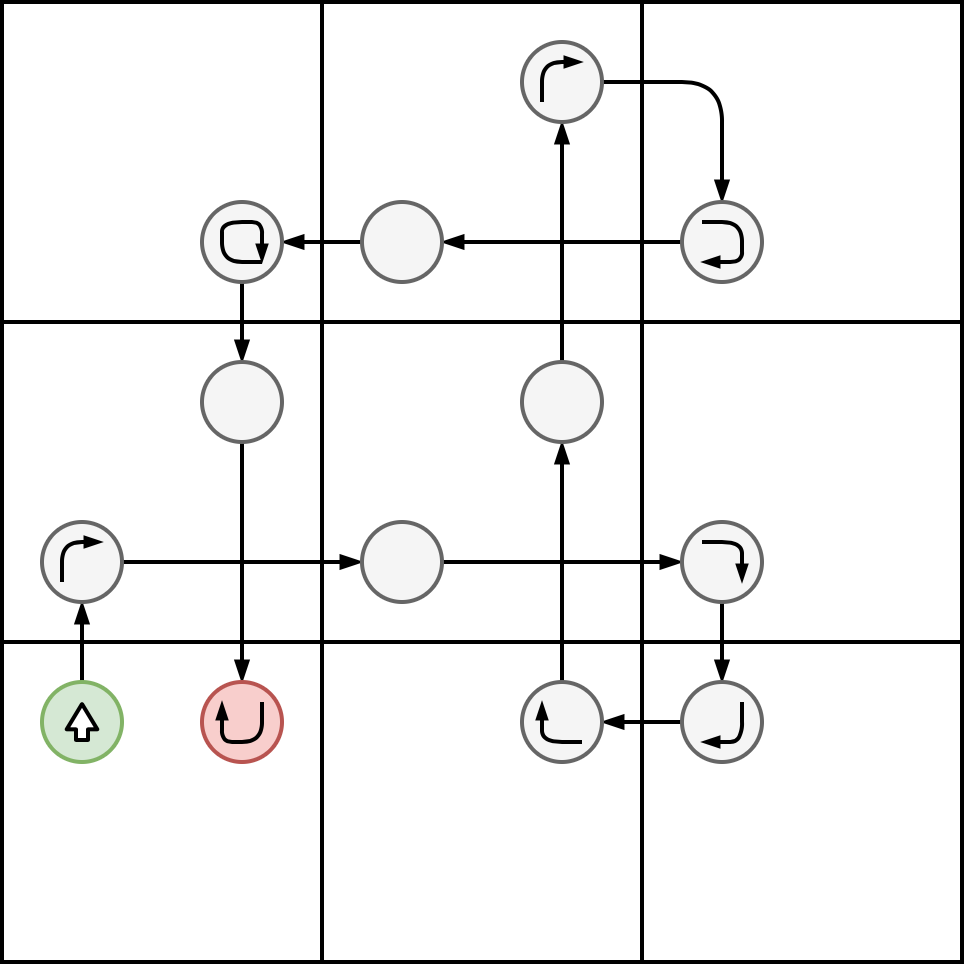
\includegraphics[scale=0.3]{vacuum3x3.png}
\caption{The shortest possible path in a 3x3 grid.}
\label{fig:vacuum3x3}
\end{figure*}

\subsection*{Task 4}

If turning takes 1 unit of time and moving forward takes 5 units of time, the fastest strategy with the given rule for (0,0) takes 26 steps -- 16 turns and 10 forwards.
This doesn't change by removing the preset rule.
It's easy to explain why this happens: since turning is much quicker than moving forward, the model prefers the path with the least amount of forward actions.
However, if turning takes more time than moving forward, the quickest strategy is always the same as the shortest.

\subsection*{Bonus task 1}

The number of forward moves is always an even number.
The number of turns is always a multiple of 4.
To find this, we had to add a final state, to avoid multiple cycles in a single verification.
Additionally, we found that the theoretical maximum number of steps in a cycle is $3\times3\times4=36$ (number of spaces times the number of directions).
\autoref{table:combinations} shows all possible combinations of forward and turn steps within one cycle.

\begin{table}[!htbp]
\centering
\begin{tabular}{|c|c|c|}
\hline
\textbf{Forward} & \textbf{Turn} & \textbf{Total} \\ \hline
12               & 12            & 24             \\ \hline
10               & 16            & 26             \\ \hline
12               & 20            & 32             \\ \hline
14               & 20            & 34             \\ \hline
\end{tabular}
\caption{The possible combinations of steps in order to achieve the goal.}
\label{table:combinations}
\end{table}

The number of turns being always a multiple of 4 explains why, when turning is slower than moving forward, the quickest path is always the shortest.
Turns always come in sets of four and the number of turns is always greater or equal to the number of forwards, so every addition of turns causes a large increase of time.

Below are some of the queries used to identify the possible combinations of steps.

\begin{verbatim}
    E<> x == 0 && y == 0 && d == n && is_clean() && n_forward == 10 && n_turn == 16
    E<> x == 0 && y == 0 && d == n && is_clean() && n_forward == 12 && n_turn == 20
    E<> x == 0 && y == 0 && d == n && is_clean() && n_forward == 14 && n_turn == 20
    E<> x == 0 && y == 0 && d == n && is_clean() && n_turn > 20
    E<> x == 0 && y == 0 && d == n && is_clean() && n_turn < 12
    E<> x == 0 && y == 0 && d == n && is_clean() && n_forward > 14
\end{verbatim}

\subsection*{Bonus task 2}

Even with all of Wooldridge's rules, the model did find a path to complete a 4x4 room.
The shortest path took 32 steps, which is illustrated in \autoref{fig:vacuum4x4}.
Removing all of the rules, the shortest path found had 28 steps.

\begin{figure*}[!htbp]
\centering
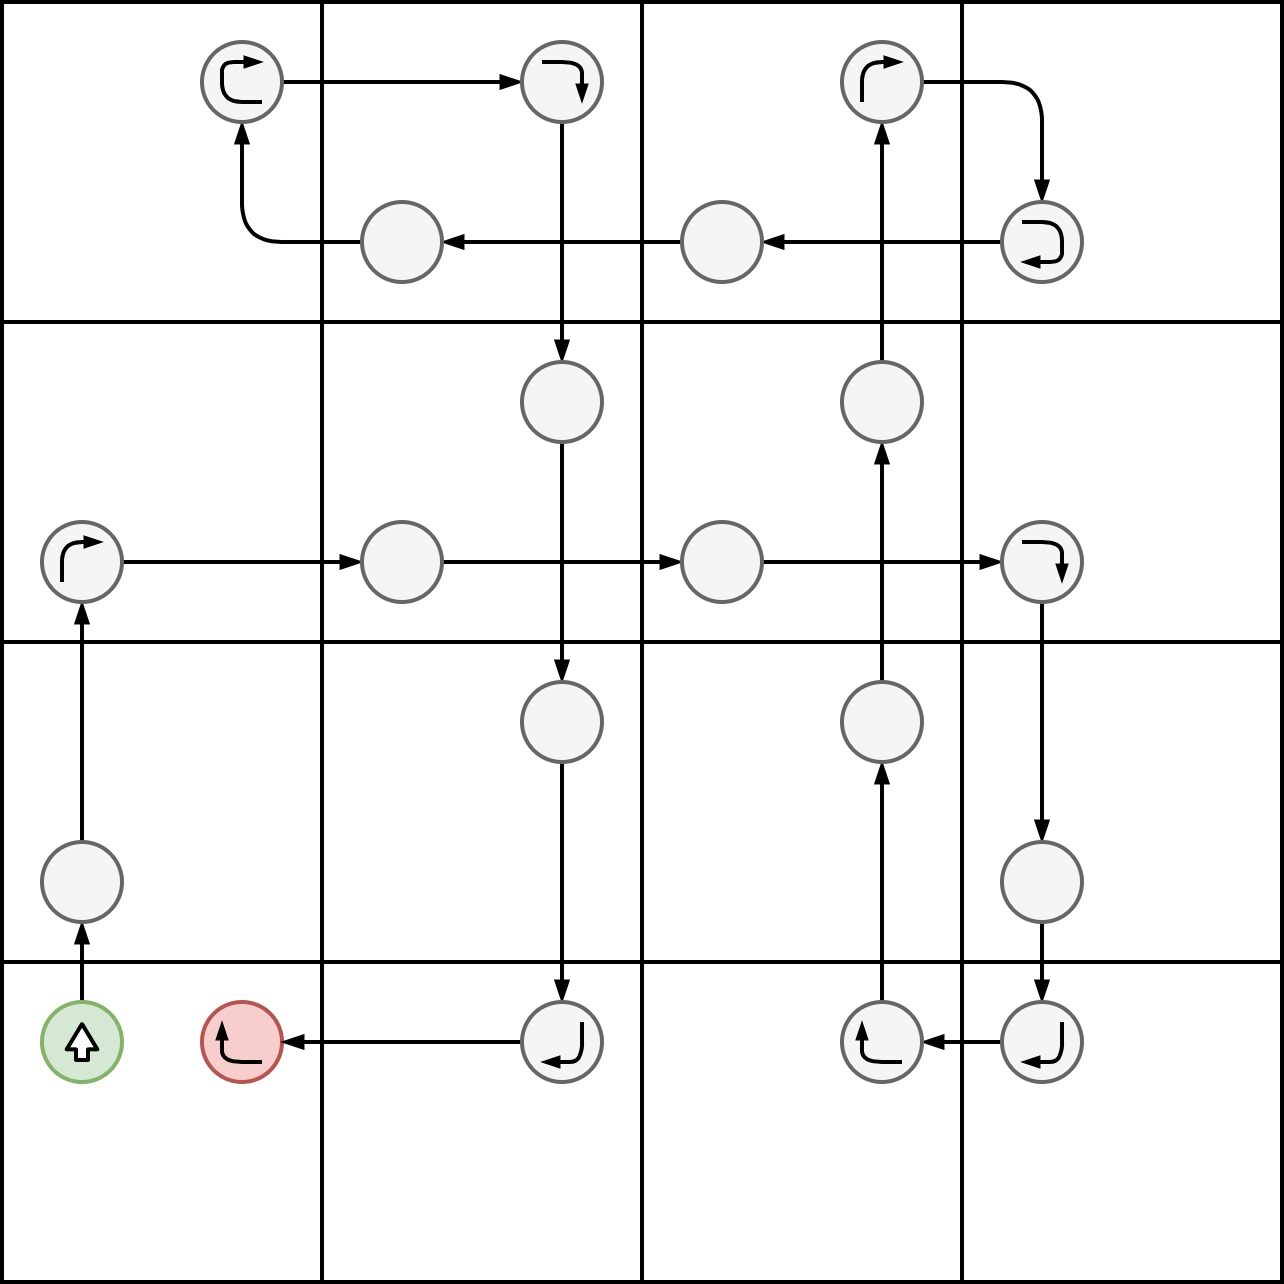
\includegraphics[scale=0.3]{vacuum4x4.png}
\caption{A path in a 4x4 grid that follows all of Wooldridge's sample rules.}
\label{fig:vacuum4x4}
\end{figure*}

\end{document}
